\documentclass[12pt, openany, oneside]{book}

\usepackage{listings}
\usepackage[dvipsnames]{xcolor}
\usepackage{ctex}
\usepackage{fontspec}
\usepackage{setspace}
\usepackage{tikz}
\usepackage{anyfontsize}
\usepackage{sectsty}
\usepackage{titlesec}
\usepackage{float}
\usepackage[hidelinks]{hyperref}
\usepackage[a4paper]{geometry}
\usepackage{url}
\usepackage{amssymb}
\usepackage{fontawesome5}
\usepackage[most]{tcolorbox}
\usepackage{circuitikz}
\usepackage{stackengine}
\usepackage{multirow}
\usepackage{newtxtt}
% \usepackage{minted}

\makeatletter
\newcommand{\verbatimfont}[1]{\renewcommand{\verbatim@font}{\ttfamily#1}}
\makeatother

\usetikzlibrary{calc,trees,positioning,arrows,fit,shapes}
\usetikzlibrary{shapes.multipart,chains}
\usetikzlibrary{automata}

\usetikzlibrary{arrows,positioning, calc,lindenmayersystems,decorations.pathmorphing,intersections}
\tikzstyle{resource}= [draw,minimum size=30pt,inner sep=0pt]
\tikzstyle{process} = [draw,minimum size=30pt,inner sep=0pt,circle]
\tikzstyle{allocated} = [->,thick,arrows={-latex}]
\tikzstyle{requested} = [<-,thick,arrows={latex-}, dashed]

\def\rlwd{.5pt} \def\rlht{2.2ex} \def\rldp{.5ex}
\def\mydiv#1{~%
  \rule[-\rldp]{\rlwd}{\rlht}%
  \setbox0=\hbox{~#1}%
  \stackunder[\dimexpr\rldp-\rlwd]{~#1}{\rule{\wd0}{\rlwd}}%
}

\definecolor{mycolor}{RGB}{0,128,128}
\newtcbox{\mybox} {
    on line,
    colback=mycolor,
    fontupper=\bfseries\color{white},
    boxrule=0pt,
    arc=5pt, 
    boxsep=0pt, 
    left=2pt, 
    right=2pt, 
    top=5pt, 
    bottom=5pt
}

\setstretch{1.5}
\setlength{\parindent}{0cm}

\geometry{a4paper,top=2.5cm,bottom=2.5cm}

\titleformat{\chapter}{\Huge\Huge\bfseries}{\chaptertitlename\ \thechapter{\ }}{0pt}{\Huge}{}
\titlespacing{\chapter}{0pt}{0pt}{12pt}

\definecolor{dkgreen}{rgb}{0,0.4,0}
\definecolor{gray}{rgb}{0.5,0.5,0.5}
\definecolor{mauve}{rgb}{0.58,0,0.82}
\definecolor{LightGray}{gray}{0.9}

\lstset{
    basicstyle=\linespread{1.3} \fontspec{Consolas},    %  the size of the fonts that are used for the code
	basewidth=0.5em,
    numbers=left,            % where to put the line-numbers
    numberstyle=\color{black},  % the style that is used for the line-numbers
    numbersep=10pt,                  % how far the line-numbers are from the code
    backgroundcolor=\color{white},
    showspaces=false,
    showstringspaces=false,
    showtabs=false,
    frame=single,                   % adds a frame around the code
    rulecolor=\color{black},        % if not set, the frame-color may be changed on line-breaks within not-black text (e.g. commens (green here))
    tabsize=4,                      % sets default tabsize to 2 spaces
    captionpos=t,                   % sets the caption-position to bottom
    breaklines=false,                % sets automatic line breaking
    breakatwhitespace=true,        % sets if automatic breaks should only happen at whitespace
    title=\lstname,                   % show the filename of files included with \lstinputlisting;
    % also try caption instead of title
    numberstyle=\color{black},		% line number color
    keywordstyle=\color{blue},          % keyword style
    commentstyle=\color{dkgreen},       % comment style
    stringstyle=\color{mauve},         % string literal style
    escapeinside={\%*}{*)},            % if you want to add LaTeX within your code
    morekeywords={*,...}               % if you want to add more keywords to the set
}

\begin{document}

\thispagestyle{empty}

\begin{tikzpicture}[overlay,remember picture]
    % Background color
    \fill[
        black!2]
    (current page.south west) rectangle (current page.north east);

    % Rectangles
    \shade[
        left color=Dandelion,
        right color=Dandelion!40,
        transform canvas ={rotate around ={45:($(current page.north west)+(0,-6)$)}}]
    ($(current page.north west)+(0,-6)$) rectangle ++(9,1.5);

    \shade[
        left color=lightgray,
        right color=lightgray!50,
        rounded corners=0.75cm,
        transform canvas ={rotate around ={45:($(current page.north west)+(.5,-10)$)}}]
    ($(current page.north west)+(0.5,-10)$) rectangle ++(15,1.5);

    \shade[
        left color=lightgray,
        rounded corners=0.3cm,
        transform canvas ={rotate around ={45:($(current page.north west)+(.5,-10)$)}}] ($(current page.north west)+(1.5,-9.55)$) rectangle ++(7,.6);

    \shade[
        left color=orange!80,
        right color=orange!60,
        rounded corners=0.4cm,
        transform canvas ={rotate around ={45:($(current page.north)+(-1.5,-3)$)}}]
    ($(current page.north)+(-1.5,-3)$) rectangle ++(9,0.8);

    \shade[
        left color=red!80,
        right color=red!80,
        rounded corners=0.9cm,
        transform canvas ={rotate around ={45:($(current page.north)+(-3,-8)$)}}] ($(current page.north)+(-3,-8)$) rectangle ++(15,1.8);

    \shade[
        left color=orange,
        right color=Dandelion,
        rounded corners=0.9cm,
        transform canvas ={rotate around ={45:($(current page.north west)+(4,-15.5)$)}}]
    ($(current page.north west)+(4,-15.5)$) rectangle ++(30,1.8);

    \shade[
        left color=RoyalBlue,
        right color=Emerald,
        rounded corners=0.75cm,
        transform canvas ={rotate around ={45:($(current page.north west)+(13,-10)$)}}]
    ($(current page.north west)+(13,-10)$) rectangle ++(15,1.5);

    \shade[
        left color=lightgray,
        rounded corners=0.3cm,
        transform canvas ={rotate around ={45:($(current page.north west)+(18,-8)$)}}]
    ($(current page.north west)+(18,-8)$) rectangle ++(15,0.6);

    \shade[
        left color=lightgray,
        rounded corners=0.4cm,
        transform canvas ={rotate around ={45:($(current page.north west)+(19,-5.65)$)}}]
    ($(current page.north west)+(19,-5.65)$) rectangle ++(15,0.8);

    \shade[
        left color=OrangeRed,
        right color=red!80,
        rounded corners=0.6cm,
        transform canvas ={rotate around ={45:($(current page.north west)+(20,-9)$)}}]
    ($(current page.north west)+(20,-9)$) rectangle ++(14,1.2);

    % Year
    % \draw[ultra thick,gray]
    % ($(current page.center)+(5,2)$) -- ++(0,-3cm)
    node[
            midway,
            left=0.25cm,
            text width=5cm,
            align=right,
            black!75
        ]
        {
            % {\fontsize{25}{30} \selectfont \bf ANNUAL \\[10pt] REPORT}
        }
    node[
            midway,
            right=0.25cm,
            text width=6cm,
            align=left,
            orange]
        {
            % {\fontsize{72}{86.4} \selectfont 2020}
        };

    % Title
    \node[align=center] at ($(current page.center)+(0,-7)$)
    {
    {\fontsize{72}{72} \selectfont {{数据库}}} \\[1cm]
    {\fontsize{42}{42} \selectfont {{Database}}} \\[2cm]
    {\fontsize{20}{19.2} \selectfont \textcolor{orange}{ \bf 极夜酱}} \\[4pt]
    };
\end{tikzpicture}

\newpage

\pagestyle{plain}
\setcounter{page}{1}
\setcounter{tocdepth}{0}
\tableofcontents

\newpage

\setcounter{page}{1}

% \chapter{数据库简介}

% \section{数据库(Database)}

% 当今的程序开发几乎都是围绕着数据库展开的,一个合理且通用的程序一定要有数据库的开发支持。 \\

% 数据库的产生最初是由IBM的一个分析人员在70年代推出的《论关系型数据库的发展》论文开始的。这篇论文一公布之后,全世界就出现了几十种不同的数据库,其中到现在还能够继续存在的数据库是Oracle,而其它的数据库要么被收购了,要么就是彻底消失了。后来IBM为了统一数据库操作,后来又推出了SQL语法结构,并且该结构也已经成为当今数据库的使用标准。

% \section{SQL(Structured Query Language)}

% SQL是一种结构化查询语言,用于数据库的访问,自1970年代诞生到现在,经久不衰,日久弥新。数据库早已遍布各个应用领域,数据管理、数据分析甚至机器学习都可以用SQL来完成。 \\

% SQL可用于在数据库中增加、删除、修改、查询数据,用于简单的数据清洗和数据分析,并可搭配其它工具制作数据报表、大数据和机器学习。 \\

% 关系数据库管理系统RDBMS(Relational Database Management System)是一种数据库软件,它将数据和数据关系以数据库和数据表的形式存储,并提供SQL访问接口。目前主流的RDBMS有MySQL、PostgreSQL、SQL Server和Oracle,其中MySQL和PostgreSQL是免费开源且使用广泛的数据库。 \\

% SQL的关键字不区分大小写,如CREATE和create的作用相同,但推荐关键字大写。SQL语句中如果包含保留词需要通过转义符转义,例如MySQL中的转义符是反引号。

% SQL是是用来操作数据的基本单位,每一条SQL语句末尾必须有分号。 \\

% SQL可以分为数据操作语言DML(Data Manipulation Language)和数据定义语言DDL(Data Definition Language)。 \\

% DDL负责数据结构定义和数据库对象定义,主要由CREATE、ALTER、DROP三个指令组成:

% \begin{table}[H]
% 	\centering
% 	\setlength{\tabcolsep}{5mm}{
% 		\begin{tabular}{|c|c|}
% 			\hline
% 			\textbf{指令}   & \textbf{功能} \\
% 			\hline
% 			CREATE DATABASE & 创建数据库    \\
% 			\hline
% 			ALTER DATABASE  & 修改数据库    \\
% 			\hline
% 			CREATE TABLE    & 创建数据表    \\
% 			\hline
% 			ALTER TABLE     & 修改数据表    \\
% 			\hline
% 			DROP DATABASE   & 删除数据库    \\
% 			\hline
% 			DROP TABLE      & 删除数据表    \\
% 			\hline
% 		\end{tabular}
% 	}
% 	\caption{DDL指令}
% \end{table}

% DML负责数据访问和数据操作,主要由INSERT、DELETE、SELECT、UPDATE组成:

% \begin{table}[H]
% 	\centering
% 	\setlength{\tabcolsep}{5mm}{
% 		\begin{tabular}{|c|c|}
% 			\hline
% 			\textbf{指令} & \textbf{功能} \\
% 			\hline
% 			SELECT FROM   & 查询数据      \\
% 			\hline
% 			UPDATE SET    & 更新数据      \\
% 			\hline
% 			DELETE FROM   & 删除数据      \\
% 			\hline
% 			INSERT INTO   & 新增数据      \\
% 			\hline
% 		\end{tabular}
% 	}
% 	\caption{DML指令}
% \end{table}

% \section{数据类型}

% 数据库之中最基本的数据管理单位是数据表,每一个数据表中会存在若干个数据列,每一种数据列都有各自对应的数据类型。 \\

% \begin{figure}[H]
% 	\centering
% 	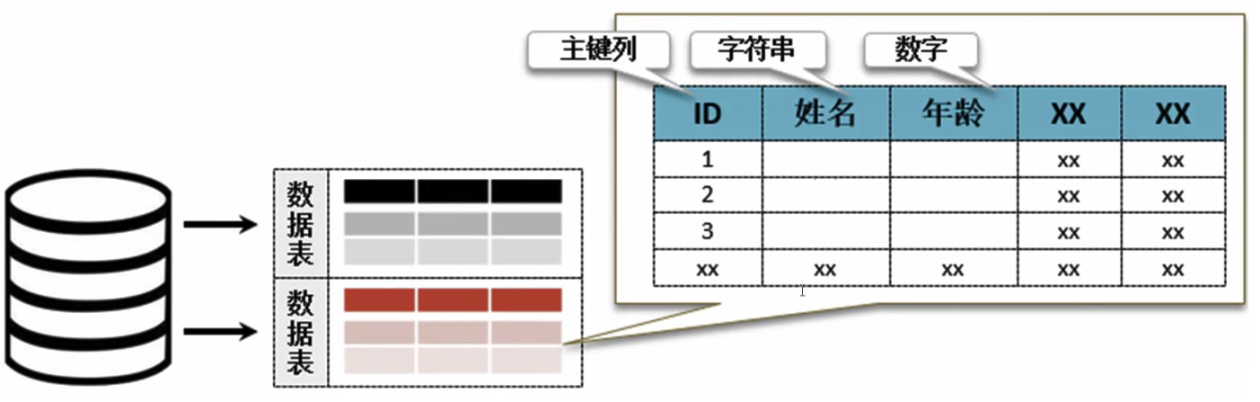
\includegraphics[]{img/C1/1.png}
% 	\caption{数据库}
% \end{figure}

% 数据表中的每个字段都需要明确地指明数据类型。常见的数据类型包括数值型、字符型和日期型。 \\

% 数值型分为整数类型和小数类型两类:

% \begin{enumerate}
% 	\item 整数类型默认有符号,无符号需要使用unsigned关键字约束,约束后不可表示负数。整数类型有数据长度的限制,如果在数据插入时超出其整型范围,数据库会报异常并插入失败。整数类型可以接受一个参数,表示它的最大显示宽度。

% 	\item 小数类型由整数部分和小数部分组成,指定时可以传入两个参数,分别表示整体的长度和小数部分的长度。
% \end{enumerate}

% \begin{table}[H]
% 	\centering
% 	\setlength{\tabcolsep}{5mm}{
% 		\begin{tabular}{|c|c|c|}
% 			\hline
% 			\textbf{数据类型} & \textbf{字节} & \textbf{描述} \\
% 			\hline
% 			tinyint(size)     & 1             & 极小整型      \\
% 			\hline
% 			smallint(size)    & 2             & 小整型        \\
% 			\hline
% 			mediumint(size)   & 3             & 中整型        \\
% 			\hline
% 			int(size)         & 4             & 整型          \\
% 			\hline
% 			bigint(size)      & 8             & 大整型        \\
% 			\hline
% 			float(size, d)    & 4             & 单精度浮点数  \\
% 			\hline
% 			double(size, d)   & 8             & 双精度浮点数  \\
% 			\hline
% 			decimal(size, d)  & 8             & 货币类型      \\
% 			\hline
% 			numeric(size, d)  & 8             & 同decimal     \\
% 			\hline
% 		\end{tabular}
% 	}
% 	\caption{数值型}
% \end{table}

% 字符类型表示文本和字符,根据字符串的长度,可以分为短文本和长文本两类。常见的短文本类型有char(不可变长)和varchar(可变长),长本文有text和blob,其中blob用来保存二进制流数据。

% \begin{table}[H]
% 	\centering
% 	\setlength{\tabcolsep}{5mm}{
% 		\begin{tabular}{|c|c|c|}
% 			\hline
% 			\textbf{数据类型} & \textbf{可否变长} & \textbf{描述}                \\
% 			\hline
% 			char(size)        & 不可              & 固定长度短字符串             \\
% 			\hline
% 			varchar(size)     & 可以              & 不固定长度短字符串           \\
% 			\hline
% 			text              & 可以              & 长字符串,保存文章内容       \\
% 			\hline
% 			blob              & 可以              & 二进制流,保存图片、媒体信息 \\
% 			\hline
% 		\end{tabular}
% 	}
% 	\caption{字符型}
% \end{table}

% \newpage

% \chapter{MySQL安装配置}

% \section{MySQL}

% MySQL是一款开源的关系型数据库,并且使用的人群众多,国内许多的开发公司为了节约软件开发成本,往往会使用大量免费开源的工具,所以MySQL这种小巧而且免费的数据库就非常受欢迎。随着MySQL版本的不断提升,很多的功能也在不断完善。 \\

% MySQL软件可直接通过官网\href{https://dev.mysql.com/downloads/mysql/8.0.html}进行下载。 \\

% \begin{figure}[H]
% 	\centering
% 	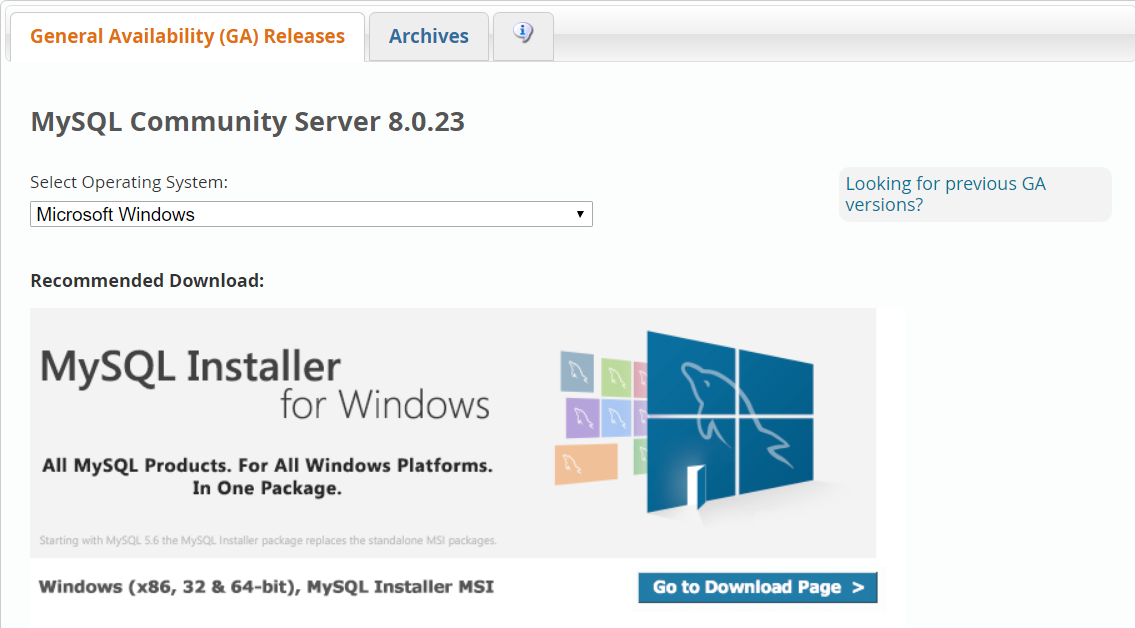
\includegraphics[scale=0.5]{img/C2/1.png}
% 	\caption{MySQL官网}
% \end{figure}

% 选择默认的Windows系统即可(尽量使用Win10系统安装,如果使用的是老系统往往需要安装大量的系统补丁)。 \\

% \begin{figure}[H]
% 	\centering
% 	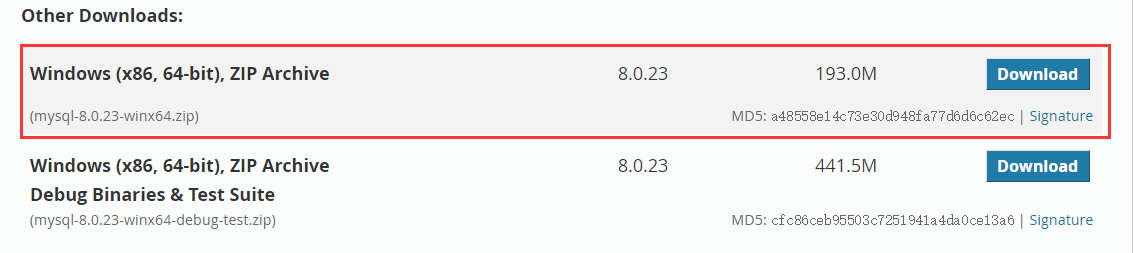
\includegraphics[scale=0.5]{img/C2/2.png}
% \end{figure}

% MySQL安装步骤:

% \subsubsection{解压缩}

% 建议将其解压缩到C盘根目录下,为了方便配置,将文件夹重命名为`mysql8`(完整路径:C:$ \backslash $mysql8)。

% \subsubsection{路径配置}

% 修改本地PATH环境属性,添加MySQL可执行文件路径。 \\

% \begin{figure}[H]
% 	\centering
% 	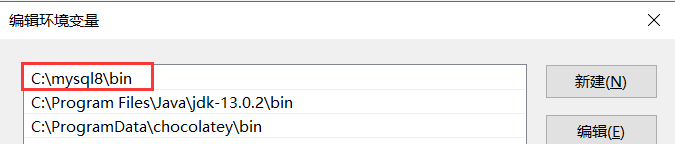
\includegraphics[]{img/C2/3.png}
% 	\caption{路径配置}
% \end{figure}

% \subsubsection{数据目录}

% MySQL所提供的仅仅是一个软件支持,但是数据库本身一定需要进行数据存储,就需要为其创建存储目录D:$ \backslash $mysql-dc$ \backslash $data和D:$ \backslash $mysql-dc$ \backslash $logs,其中data保存真实数据,logs保存相关日志。

% \subsubsection{MySQL配置}

% 通过配置文件my.ini建立C:$ \backslash $mysql8和D:$ \backslash $mysql-dc两个目录之间的联系。 \\

% \begin{figure}[H]
% 	\centering
% 	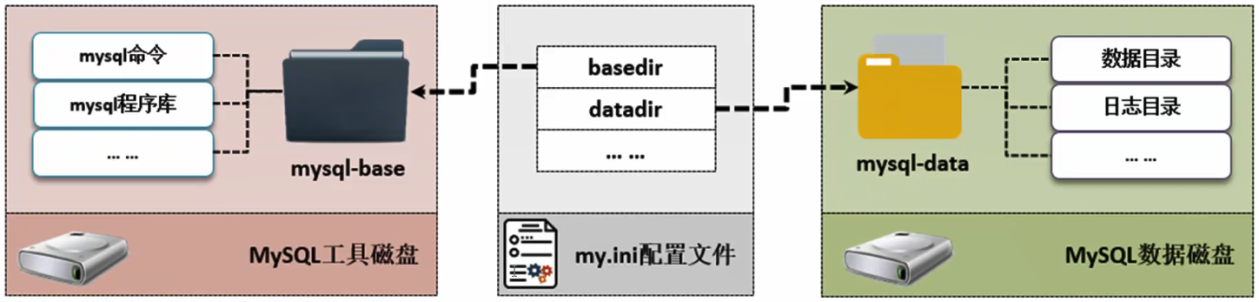
\includegraphics[]{img/C2/4.png}
% 	\caption{MySQL配置}
% \end{figure}

% \mybox{创建my.ini文件}

% \begin{lstlisting}
% [mysqld]
% # 设置3306端口
% port=3306
% # 设置mysql的安装目录
% basedir=C:\mysql8
% # 设置mysql数据库的数据的存放目录
% datadir=D:\mysql-dc\data
% # mysqlsock存储目录
% socket=D:\mysql-dc\data\mysql.sock
% # 允许最大连接数
% max_connections=10000
% # 允许连接失败的次数。这是为了防止有人从该主机试图攻击数据库系统
% max_connect_errors=10
% # 服务端使用的字符集默认为UTF8
% character-set-server=UTF8MB4
% # 创建新表时将使用的默认存储引擎
% default-storage-engine=INNODB
% # 默认使用"mysql_native_password"插件认证
% default_authentication_plugin=mysql_native_password
% [mysql]
% # 设置mysql客户端默认字符集
% default-character-set=UTF8MB4
% # mysqlsock存储目录
% socket=D:\mysql-dc\data\mysql.sock
% [client]
% # 设置mysql客户端连接服务端时默认使用的端口
% port=3306
% default-character-set=utf8
% [mysqld_safe]
% log-error=D:\mysql-dc\logs\mysql.log
% pid-file=D:\mysql-dc\logs\mysql.pid
% # mysqlsock存储目录
% socket=D:\mysql-dc\data\mysql.sock
% \end{lstlisting}

% \subsubsection{数据库初始化}

% 在命令行中通过MySQL提供的命令生成结构性文件,数据库初始化的时候会自动生成一个临时的密码,在没有修改之前只能通过此密码进行MySQL数据库的访问。 \\

% \mybox{数据库初始化}

% \begin{lstlisting}
% mysqld --initialize --console
% \end{lstlisting}

% \begin{tcolorbox}
% 	\mybox{临时密码}
% 	\begin{verbatim}
% ah+K3SB2,B(B
% 	\end{verbatim}
% \end{tcolorbox}

% \subsubsection{服务安装}

% 将MySQL启动命令添加到服务之中。在进行服务安装的时候一般都需要管理员的操作权限,所以一定要以管理员的身份打开命令行工具,否则会出现Install/Remove of the Service Denied!错误信息。 \\

% \mybox{安装并开启服务}

% \begin{lstlisting}
% mysqld install
% net start mysql
% \end{lstlisting}

% \subsubsection{服务登录}

% 通过命令行的模式进行MySQL数据库登录。第一次密码为系统初始化时生成的临时密码。 \\

% \mybox{MySQL登录}

% \begin{lstlisting}
% mysql -uroot -pah+K3SB2,B(B
% \end{lstlisting}

% \subsubsection{修改密码}

% 将临时密码修改为自己的密码,将root超级管理员的密码设置为mysqladmin。 \\

% \mybox{修改密码}

% \begin{lstlisting}[language=SQL]
% alter user 'root'@'localhost' IDENTIFIED WITH mysql_native_password
% BY 'mysqladmin';
% \end{lstlisting}

% \subsubsection{远程登录配置}

% 此时的root账户只能够在本地进行登录访问,所以需要开启远程访问配置。 \\

% \mybox{远程登录配置}

% \begin{lstlisting}[language=SQL]
% # 进入配置数据库
% use mysql
% # 设置远程访问
% update user set user.Host='%' where user.User='root';
% # 配置立即生效
% flush privileges;
% \end{lstlisting}

% MySQL数据库需要通过命令的模式来完成,要想使用MySQL数据库就必须通过用户名和密码进行数据库的登录。 \\

% \mybox{数据库登录}

% \begin{lstlisting}[language=SQL]
% mysql -uroot -pmysqladmin
% \end{lstlisting}

% 在一个数据库平台上会存在许多的数据库,通过SHOW DATABASES;可以查看当前环境下所有已经存在的数据库信息。 \\

% \mybox{查看数据库}

% \begin{lstlisting}[language=SQL]
% SHOW DATABASES;
% \end{lstlisting}

% \begin{tcolorbox}
% 	\mybox{运行结果}
% 	\begin{verbatim}
% +--------------------+
% | Database           |
% +--------------------+
% | information_schema |
% | mysql              |
% | performance_schema |
% | sys                |
% +--------------------+
% 	\end{verbatim}
% \end{tcolorbox}

% \newpage

% \chapter{CREATE}

% \section{创建数据库}

% CREATE负责数据库对象的创建,数据库、数据表、数据库索引、函数等都可以使用CREATE来创建。 \\

% 既然在一个平台上会有许多的数据库,那么在使用的时候就必须明确地确定好一个数据库,通过USE命令来进行数据库的使用切换。

% \vspace{-0.5cm}

% \begin{lstlisting}[language=SQL]
% CREATE DATABASE [database_name];
% USE [database_name];
% \end{lstlisting}

% \vspace{0.5cm}

% \mybox{创建student数据库}

% \begin{lstlisting}[language=SQL]
% CREATE DATABASE student;
% USE student;
% \end{lstlisting}

% SQL语句可以保存到.sql脚本中,在连接MySQL数据库后使用source指定脚本路径。

% \vspace{-0.5cm}

% \begin{lstlisting}[language=SQL]
% source [path]
% \end{lstlisting}

% \section{创建数据表}

% CREATE TABLE指令可以在数据库中创建数据表。通过DESC指令可以查看数据表结构。

% \vspace{-0.5cm}

% \begin{lstlisting}[language=SQL]
% CREATE TABLE [table_name](
%     [col1] [datatype1],
%     [col2] [datatype2],
%     [col3] [datatype3],
%     ....
% );

% DESC [table_name];
% \end{lstlisting}

% \vspace{0.5cm}

% \mybox{创建数据表} \\

% 创建info数据表,字段包括id、name、gpa。

% \vspace{-0.5cm}

% \begin{lstlisting}[language=SQL]
% CREATE TABLE info(
%     id int, 
%     name varchar(16), 
%     gpa double(5, 2)
% );

% DESC info;
% \end{lstlisting}

% \begin{tcolorbox}
% 	\mybox{运行结果}
% 	\begin{verbatim}
% +-------+-------------+------+-----+---------+-------+
% | Field | Type        | Null | Key | Default | Extra |
% +-------+-------------+------+-----+---------+-------+
% | id    | int         | YES  |     | NULL    |       |
% | name  | varchar(16) | YES  |     | NULL    |       |
% | gpa   | double(5,2) | YES  |     | NULL    |       |
% +-------+-------------+------+-----+---------+-------+
% 	\end{verbatim}
% \end{tcolorbox}

% NULL是对未知/缺失属性的标识,常用于表示某个字段为空,NULL是所有可以为空字段的默认值。 \\

% NULL必须使用运算符IS和IS NOT进行比较。NULL与0并不是等价的,它们无法比较。

% \section{约束(Constraint)}

% SQL约束用于在新建或修改数据表时,给数据表或数据表中的字段加上约束条件。约束既可以在字段上,也可以在表上。一个字段,或者一张表可以有多个约束。

% \vspace{-0.5cm}

% \begin{lstlisting}[language=SQL]
% CREATE TABLE [table_name](
%     [col1] [datatype1] [constraint1],
%     [col2] [datatype2] [constraint2],
%     [col3] [datatype3] [constraint3],
%     ....,
%     [constraint4]
% );
% \end{lstlisting}

% \begin{table}[H]
% 	\centering
% 	\setlength{\tabcolsep}{5mm}{
% 		\begin{tabular}{|c|c|}
% 			\hline
% 			\textbf{约束} & \textbf{功能} \\
% 			\hline
% 			NOT NULL      & 字段非空      \\
% 			\hline
% 			DEFAULT       & 字段默认值    \\
% 			\hline
% 			UNIQUE        & 字段唯一      \\
% 			\hline
% 			PRIMARY KEY   & 主键          \\
% 			\hline
% 			FOREIGN KEY   & 外键          \\
% 			\hline
% 			CHECK         & 校验字段      \\
% 			\hline
% 		\end{tabular}
% 	}
% 	\caption{约束}
% \end{table}

% \begin{itemize}
% 	\item DEFAULT会给字段添加上默认值,若字段在添加的时候没有指定值,则使用默认值。

% 	\item NOT NULL表示一个字段是非空的,当在插入或者修改时,如果字段为空则报错。

% 	\item PRIMARY KEY表示主键,用于唯一标识数据表中的每一条记录。主键不能为空,并且必须是唯一的,即每条记录的主键必须各不相同。

% 	\item UNIQUE用于唯一数据表中的每一条记录,UNIQUE约束的字段必须是唯一的,即该字段在每条记录中必须各不相同。PRIMARY KEY约束默认拥有UNIQUE约束。每个表可以有多个UNIQUE约束,但是只能有一个PRIMARY KEY。
% \end{itemize}

% 在数据表已经存在的情况下不能重复创建同名表,因此需要使用DROP语句删除已经存在的数据表。 \\

% \mybox{约束} \\

% 创建info数据表,字段包括id、name、gpa,其中id为主键,name为非空字段,gpa默认为0。

% \vspace{-0.5cm}

% \begin{lstlisting}[language=SQL]
% DROP TABLE IF EXISTS info;

% CREATE TABLE info(
%     id int PRIMARY KEY,
%     name varchar(16) NOT NULL,
%     gpa double(5, 2) DEFAULT 0
% );

% DESC info;
% \end{lstlisting}

% \begin{tcolorbox}
% 	\mybox{运行结果}
% 	\begin{verbatim}
% +-------+-------------+------+-----+---------+-------+
% | Field | Type        | Null | Key | Default | Extra |
% +-------+-------------+------+-----+---------+-------+
% | id    | int         | NO   | PRI | NULL    |       |
% | name  | varchar(16) | NO   |     | NULL    |       |
% | gpa   | double(5,2) | YES  |     | 0.00    |       |
% +-------+-------------+------+-----+---------+-------+
%     \end{verbatim}
% \end{tcolorbox}

% \section{CHECK}

% CHECK约束用于限制字段值的范围,既可以定义在单个字段上,也可以在定义在表上对特定字段进行约束。CHECK可以在数据库层面上筛选掉不符合约束的数据。创建成功后,若插入的数据不满足条件,会导致插入失败。 \\

% \mybox{CHECK} \\

% 创建数据表info,包括id、name、age三个,age字段添加CHECK约束,规定所有age必须大于0。

% \vspace{-0.5cm}

% \begin{lstlisting}[language=SQL]
% DROP TABLE IF EXISTS info;

% CREATE TABLE info(
%     id int,
%     name varchar(20),
%     age int unsigned CHECK(age > 0)
% );

% DESC info;
% \end{lstlisting}

% \begin{tcolorbox}
% 	\mybox{运行结果}
% 	\begin{verbatim}
% +-------+--------------+------+-----+---------+-------+
% | Field | Type         | Null | Key | Default | Extra |
% +-------+--------------+------+-----+---------+-------+
% | id    | int          | YES  |     | NULL    |       |
% | name  | varchar(20)  | YES  |     | NULL    |       |
% | age   | int unsigned | YES  |     | NULL    |       |
% +-------+--------------+------+-----+---------+-------+
%     \end{verbatim}
% \end{tcolorbox}

% \newpage

% \chapter{ALTER}

% \section{初始数据}

% \mybox{初始数据}

% \begin{lstlisting}[language=SQL]
% DROP TABLE IF EXISTS info;

% CREATE TABLE info(
%     id int, 
%     name varchar(16), 
%     gpa double(5, 2)
% );
% \end{lstlisting}

% \section{ALTER}

% ALTER指令用于已有数据表的修改,增加、修改和删除数据表字段都可以通过ALTER来完成。ALTER使用户可以修改已创建的数据表,但大多数情况下数据表字段和类型需要在定义的时候就确认,ALTER修改数据表是非常消耗性能和时间的。 \\

% 添加、删除、修改字段语法如下:

% \vspace{-0.5cm}

% \begin{lstlisting}[language=SQL]
% ALTER TABLE [table_name] ADD ([col] [datatype]);
% ALTER TABLE [table_name] DROP [col];
% ALTER TABLE [table_name] MODIFY (COLUMN [col] [datatype] [constraint]);
% \end{lstlisting}

% \vspace{0.5cm}

% \mybox{ALTER} \\

% 为info表添加字段phone,类型为varchar(20);删除字段gpa;修改字段id类型为varchar(10),字段非空。

% \vspace{-0.5cm}

% \begin{lstlisting}[language=SQL]
% ALTER TABLE info ADD phone varchar(20);
% ALTER TABLE info DROP gpa;
% ALTER TABLE info MODIFY id varchar(10) NOT NULL;
% DESC info;
% \end{lstlisting}

% \begin{tcolorbox}
% 	\mybox{运行结果}
% 	\begin{verbatim}
% +-------+-------------+------+-----+---------+-------+
% | Field | Type        | Null | Key | Default | Extra |
% +-------+-------------+------+-----+---------+-------+
% | id    | varchar(10) | NO   |     | NULL    |       |
% | name  | varchar(16) | YES  |     | NULL    |       |
% | phone | varchar(20) | YES  |     | NULL    |       |
% +-------+-------------+------+-----+---------+-------+
%     \end{verbatim}
% \end{tcolorbox}

% \newpage

% \chapter{DROP}

% \section{DROP}

% DROP指令用于删除数据库、数据表、索引和视图等,DROP强大而又危险,它能迅速清理掉数据库垃圾,不过使用之前请仔细斟酌,删除的数据很可能再也找不回来了。DROP几乎可以清理掉数据库中的任何对象,因此在操作之前必须确保数据的安全性。 \\

% 删除数据库、诉苦表语法如下:

% \vspace{-0.5cm}

% \begin{lstlisting}[language=SQL]
% DROP DATABASE [db_name];
% DROP TABLE [table_name];
% \end{lstlisting}

% TRUNCATE指令可以在保留数据表的情况下清空数据表数据。

% \vspace{-0.5cm}

% \begin{lstlisting}[language=SQL]
% TRUNCATE TABLE [table_name];
% \end{lstlisting}

% \newpage

% \chapter{INSERT}

% \section{初始数据}

% \mybox{初始数据}

% \begin{lstlisting}[language=SQL]
% DROP TABLE IF EXISTS info;

% CREATE TABLE info(
%     id int,
%     name varchar(16),
%     gpa double(5, 2)
% );
% \end{lstlisting}

% \section{INSERT}

% INSERT指令用于向数据表中添加记录,INSERT插入数据分为普通插入和批量插入。并不是每个RDBMS都支持批量插入,批量插入的移植性并不好,如果所使用的数据库不支持,可以将其改为多个普通插入。

% \vspace{-0.5cm}

% \begin{lstlisting}[language=SQL]
% INSERT INTO [table_name] ([col1], [col2]) VALUES([val1], [val2]);
% \end{lstlisting}

% 如果插入的数据是全字段,那么可以省略前面的col。

% \vspace{-0.5cm}

% \begin{lstlisting}[language=SQL]
% INSERT INTO [table_name] VALUES([val1], [val2]);
% \end{lstlisting}

% \vspace{0.5cm}

% \mybox{单条插入} \\

% 向数据表info中插入一条记录,id为1,name为Terry,gpa为3.7。

% \vspace{-0.5cm}

% \begin{lstlisting}[language=SQL]
% INSERT INTO info VALUES(1, "Terry", 3.7);
% SELECT * FROM info;
% \end{lstlisting}

% \begin{tcolorbox}
% 	\mybox{运行结果}
% 	\begin{verbatim}
% +------+-------+------+
% | id   | name  | gpa  |
% +------+-------+------+
% |    1 | Terry | 3.70 |
% +------+-------+------+
%     \end{verbatim}
% \end{tcolorbox}

% 批量插入与普通插入的区别在于,VALUES关键字后面接受多个字段元组,每个()代表一个字段元组,一个字段元组会生成一条记录。

% \vspace{-0.5cm}

% \begin{lstlisting}[language=SQL]
% INSERT INTO [table_name] ([col1], [col2]) VALUES
% ([val1], [val2]),
% ([val1], [val2]);
% \end{lstlisting}

% \vspace{0.5cm}

% \mybox{批量插入} \\

% 向info表中插入两条记录,第一条记录\{2, "Lily", 4.2\},第二条记录\{3, "Eric", 3.3\}。

% \vspace{-0.5cm}

% \begin{lstlisting}[language=SQL]
% INSERT INTO info VALUES (2, "Lily", 4.2), (3, "Eric", 3.3);
% SELECT * FROM info;
% \end{lstlisting}

% \begin{tcolorbox}
% 	\mybox{运行结果}
% 	\begin{verbatim}
% +------+-------+------+
% | id   | name  | gpa  |
% +------+-------+------+
% |    1 | Terry | 3.70 |
% |    2 | Lily  | 4.20 |
% |    3 | Eric  | 3.30 |
% +------+-------+------+
%     \end{verbatim}
% \end{tcolorbox}

% \newpage

% \chapter{SELECT}

% \section{初始数据}

% \mybox{初始数据}

% \begin{lstlisting}[language=SQL]
% DROP TABLE IF EXISTS info;

% CREATE TABLE info(
%     id int,
%     name varchar(16),
%     gpa double(5, 2)
% );

% INSERT INTO info VALUES
% (1, "Terry", 3.7),
% (2, "Lily", 4.2),
% (3, "Eric", 3.3),
% (4, "Alice", 3.6),
% (5, "Lily", 4.2),
% (6, "Terry", 3.7),
% (7, "Anna", 4.1),
% (8, "Jason", 3.9);
% \end{lstlisting}

% \section{查询数据库信息}

% SELECT指令用于查询数据库中的数据,通过SELECT可以快速获取数据库中的变量和信息。 \\

% \mybox{查询数据库信息}

% \begin{lstlisting}[language=SQL]
% SELECT version();
% SELECT current_user;
% \end{lstlisting}

% \begin{tcolorbox}
%     \mybox{运行结果}
%     \begin{verbatim}
% +-----------+
% | version() |
% +-----------+
% | 8.0.26    |
% +-----------+

% +--------------+
% | current_user |
% +--------------+
% | root@%       |
% +--------------+
%     \end{verbatim}
% \end{tcolorbox}

% \section{查询数据表数据}

% 大部分情况下,SELECT都是用来获取数据表数据。

% \vspace{-0.5cm}

% \begin{lstlisting}[language=SQL]
% SELECT [col1], [col2] FROM [table_name];
% \end{lstlisting}

% SELECT后面跟的是要查询的字段名,若是查询所有字段,可以使用【*】表示。但是即使是获取全字段,也不推荐使用【*】,显式地给出查询字段,更容易维护和合作。

% \vspace{-0.5cm}

% \begin{lstlisting}[language=SQL]
% SELECT * FROM [table_name];
% \end{lstlisting}

% \vspace{0.5cm}

% \mybox{查询info表中name和gpa字段}

% \begin{lstlisting}[language=SQL]
% SELECT name, gpa FROM info;
% \end{lstlisting}

% \begin{tcolorbox}
%     \mybox{运行结果}
%     \begin{verbatim}
% +-------+------+
% | name  | gpa  |
% +-------+------+
% | Terry | 3.70 |
% | Lily  | 4.20 |
% | Eric  | 3.30 |
% | Alice | 3.60 |
% | Lily  | 4.20 |
% | Terry | 3.70 |
% | Anna  | 4.10 |
% | Jason | 3.90 |
% +-------+------+
%     \end{verbatim}
% \end{tcolorbox}

% 有时查询出来的所有数据会很多,SELECT在查询的时候可以使用LIMIT指定条数。

% \vspace{-0.5cm}

% \begin{lstlisting}[language=SQL]
% SELECT [col1], [col2] FROM [table_name] LIMIT n;
% \end{lstlisting}

% 有时想要查询指定起始位置指定条数的结果集,起始位置默认为0。

% \vspace{-0.5cm}

% \begin{lstlisting}[language=SQL]
% SELECT [col1], [col2] FROM [table_name] LIMIT start_pos, n;
% \end{lstlisting}

% 使用AS指令可以为表名或列明指定别名, 在显示结果时使字段名称更具有可读性。 \\

% \mybox{查询info表中前4条数据}

% \begin{lstlisting}[language=SQL]
% SELECT name AS student_name, gpa FROM info LIMIT 4;
% \end{lstlisting}

% \begin{tcolorbox}
%     \mybox{运行结果}
%     \begin{verbatim}
% +--------------+------+
% | student_name | gpa  |
% +--------------+------+
% | Terry        | 3.70 |
% | Lily         | 4.20 |
% | Eric         | 3.30 |
% | Alice        | 3.60 |
% +--------------+------+
%     \end{verbatim}
% \end{tcolorbox}

% \section{DISTINCT}

% 有时候查询结果中会包含重复的信息,DISTINCT关键字用于返回去重后的数据,但是DISTINCT去掉重复值带来的时间损耗比查询本身更耗时。DISTINCT既可以用来修饰单字段,也可以用来修饰多字段。

% \vspace{-0.5cm}

% \begin{lstlisting}[language=SQL]
% SELECT DISTINCT [col1], [col2] FROM [table_name];
% \end{lstlisting}

% \vspace{0.5cm}

% \mybox{去除info表中重复记录}

% \begin{lstlisting}[language=SQL]
% SELECT DISTINCT name, gpa FROM info;
% \end{lstlisting}

% \begin{tcolorbox}
%     \mybox{运行结果}
%     \begin{verbatim}
% +-------+------+
% | name  | gpa  |
% +-------+------+
% | Terry | 3.70 |
% | Lily  | 4.20 |
% | Eric  | 3.30 |
% | Alice | 3.60 |
% | Anna  | 4.10 |
% | Jason | 3.90 |
% +-------+------+
%     \end{verbatim}
% \end{tcolorbox}

% \section{WHERE}

% 数据表中的数据往往比较繁杂,在查询的时候需要按照一定的条件进行筛选,WHERE指令用于筛选出满足条件的结果集。WHERE后仅有一个条件子句的查询称为单条件查询。

% \vspace{-0.5cm}

% \begin{lstlisting}[language=SQL]
% SELECT [col1], [col2] from [table_name] WHERE [col] [condition] [val];
% \end{lstlisting}

% \begin{table}[H]
%     \centering
%     \setlength{\tabcolsep}{5mm}{
%         \begin{tabular}{|c|c|c|c|}
%             \hline
%             \textbf{运算符} & \textbf{功能} & \textbf{运算符} & \textbf{功能} \\
%             \hline
%             >               & 大于          & >=              & 大于等于      \\
%             \hline
%             <               & 小于          & <=              & 小于等于      \\
%             \hline
%             =               & 等于          & !=、<>          & 不等于        \\
%             \hline
%             !>              & 不大于        & !<              & 不小于        \\
%             \hline
%             AND             & 与            & OR              & 或            \\
%             \hline
%         \end{tabular}
%     }
%     \caption{运算符}
% \end{table}

% \mybox{查询info表中gpa在3.3 $ \sim $ 3.5之间的学生}

% \begin{lstlisting}[language=SQL]
% SELECT * from info WHERE gpa >= 3.3 AND gpa <= 3.6;
% \end{lstlisting}

% \begin{tcolorbox}
%     \mybox{运行结果}
%     \begin{verbatim}
% +------+-------+------+
% | id   | name  | gpa  |
% +------+-------+------+
% |    3 | Eric  | 3.30 |
% |    4 | Alice | 3.60 |
% +------+-------+------+
%     \end{verbatim}
% \end{tcolorbox}

% \newpage

% \chapter{ORDER BY}

% \section{初始数据}

% \mybox{初始数据}

% \begin{lstlisting}[language=SQL]
% DROP TABLE IF EXISTS info;

% CREATE TABLE info(
%     id int,
%     name varchar(20),
%     gpa double(5, 2)
% );

% INSERT INTO info VALUES
% (6, "Tina", 3.7),
% (1, "Terry", 3.7),
% (2, "Lily", 4.2),
% (5, "Harry", 4.2),
% (4, "Alice", 3.6),
% (8, "Jason", 3.9),
% (3, "Eric", 3.3),
% (7, "Anna", 4.1);
% \end{lstlisting}

% \section{ORDER BY}

% ORDER BY可以根据一个或多个字段对结果集排序,默认按照ASC升序排序,降序排序可以指定DESC。 \\

% 多字段排序会优先以第一字段排序后,再排序第二字段。ORDER BY对于多字段的排序支持虽然强大,但是很消耗性能。

% \vspace{-0.5cm}

% \begin{lstlisting}[language=SQL]
% SELECT [col] FROM [table_name]
% ORDER BY [col1] [DESC|ASC], [col2] [DESC|ASC];
% \end{lstlisting}

% \vspace{0.5cm}

% \mybox{ORDER BY} \\

% 将info表中的学生按照gpa降序排序,gpa相同时以id升序排序。

% \vspace{-0.5cm}

% \begin{lstlisting}[language=SQL]
% SELECT * FROM info ORDER BY gpa DESC, id ASC;
% \end{lstlisting}

% \begin{tcolorbox}
%     \mybox{运行结果}
%     \begin{verbatim}
% +------+-------+------+
% | id   | name  | gpa  |
% +------+-------+------+
% |    2 | Lily  | 4.20 |
% |    5 | Harry | 4.20 |
% |    7 | Anna  | 4.10 |
% |    8 | Jason | 3.90 |
% |    1 | Terry | 3.70 |
% |    6 | Tina  | 3.70 |
% |    4 | Alice | 3.60 |
% |    3 | Eric  | 3.30 |
% +------+-------+------+
%     \end{verbatim}
% \end{tcolorbox}

% \newpage

% \chapter{UPDATE}

% \section{初始数据}

% \mybox{初始数据}

% \begin{lstlisting}[language=SQL]
% DROP TABLE IF EXISTS info;

% CREATE TABLE info(
%     id int,
%     name varchar(16),
%     gpa double(5, 2)
% );

% INSERT INTO info VALUES
% (1, "Terry", 3.7),
% (2, "Lily", 4.2),
% (3, "Eric", 3.3);
% \end{lstlisting}

% \section{UPDATE}

% UPDATE指令用于更新数据库,一般情况下UPDATE会和WHERE搭配使用。

% \vspace{-0.5cm}

% \begin{lstlisting}[language=SQL]
% UPDATE [table_name] SET [col] = [val] WHERE [col] = [val];
% \end{lstlisting}

% \vspace{0.5cm}

% \mybox{UPDATE} \\

% 在info表中,将Eric的姓名改为Kris,gpa改为3.4。

% \vspace{-0.5cm}

% \begin{lstlisting}[language=SQL]
% UPDATE info SET name = "Kris", gpa = 3.4 WHERE name = "Eric";
% SELECT * FROM info;
% \end{lstlisting}

% \begin{tcolorbox}
%     \mybox{运行结果}
%     \begin{verbatim}
% +------+-------+------+
% | id   | name  | gpa  |
% +------+-------+------+
% |    1 | Terry | 3.70 |
% |    2 | Lily  | 4.20 |
% |    3 | Kris  | 3.40 |
% +------+-------+------+
%     \end{verbatim}
% \end{tcolorbox}

% \newpage

% \chapter{DELETE}

% \section{初始数据}

% \mybox{初始数据}

% \begin{lstlisting}[language=SQL]
% DROP TABLE IF EXISTS info;

% CREATE TABLE info(
%     id int,
%     name varchar(16),
%     gpa double(5, 2)
% );

% INSERT INTO info VALUES
% (1, "Terry", 3.7),
% (2, "Lily", 4.2),
% (3, "Eric", 3.3);
% \end{lstlisting}

% \section{DELETE}

% DELETE指令用于删除数据库中的数据,一般情况下DELETE会和WHERE一起搭配使用,来删除指定数据。 \\

% DELETE删除的单位是行,即一条记录,而不是用于删除某个字段。

% \vspace{-0.5cm}

% \begin{lstlisting}[language=SQL]
% DELETE FROM [table_name] WHERE [col] = [val];
% \end{lstlisting}

% 切勿直接使用DELETE FROM [table\_name],这样会直接删除所有的数据。删除数据是一个危险操作,在使用前请慎重考虑。 \\

% \mybox{在info表中删除Eric的记录}

% \begin{lstlisting}[language=SQL]
% DELETE FROM info WHERE name = "Eric";
% SELECT * FROM info;
% \end{lstlisting}

% \begin{tcolorbox}
%     \mybox{运行结果}
%     \begin{verbatim}
% +------+-------+------+
% | id   | name  | gpa  |
% +------+-------+------+
% |    1 | Terry | 3.70 |
% |    2 | Lily  | 4.20 |
% +------+-------+------+
%     \end{verbatim}
% \end{tcolorbox}

% \newpage

% \chapter{LIKE \& REGEXP}

% \section{初始数据}

% \mybox{初始数据}

% \begin{lstlisting}[language=SQL]
% DROP TABLE IF EXISTS info;

% CREATE TABLE info(
%     id int,
%     name varchar(16),
%     gpa double(5, 2)
% );

% INSERT INTO info VALUES
% (1, "Terry", 3.7),
% (2, "Lily", 4.2),
% (3, "Eric", 3.3),
% (4, "Alice", 3.6),
% (5, "Anna", 4.1),
% (6, "Henry", 3.9);
% \end{lstlisting}

% \section{LIKE}

% 很多时候数据表中存储了大量的字符类型字段,LIKE操作符可用于搜索和匹配字符字段。LIKE一般与WHERE搭配使用,表示搜索像某个值的字段。

% \vspace{-0.5cm}

% \begin{lstlisting}[language=SQL]
% SELECT [col] FROM [table_name] WHERE [col] LIKE [val];
% \end{lstlisting}

% 通配符是用特殊的字符来表示一个或多个字符,通配符必须和LIKE搭配使用。

% \begin{table}[H]
%     \centering
%     \setlength{\tabcolsep}{5mm}{
%         \begin{tabular}{|c|c|}
%             \hline
%             \textbf{运算符}  & \textbf{功能}                \\
%             \hline
%             \%               & 匹配一个或多个字符           \\
%             \hline
%             \_               & 匹配一个字符                 \\
%             \hline
%             [char\_list]     & 匹配列表中的任意一个字符     \\
%             \hline
%             [\^{}char\_list] & 匹配不在列表中的任意一个字符 \\
%             \hline
%         \end{tabular}
%     }
%     \caption{通配符}
% \end{table}

% 注意,MySQL与PostgreSQL均不支持字符列表通配符,在实际场景中可以使用正则(REGEXP)来替代。 \\

% \mybox{LIKE} \\

% 在info表中匹配出所有name中第二个字符为e,并且以y结尾的学生。

% \vspace{-0.5cm}

% \begin{lstlisting}[language=SQL]
% SELECT * FROM info WHERE name LIKE "_e%y";
% \end{lstlisting}

% \begin{tcolorbox}
%     \mybox{运行结果}
%     \begin{verbatim}
% +------+-------+------+
% | id   | name  | gpa  |
% +------+-------+------+
% |    1 | Terry | 3.70 |
% |    6 | Henry | 3.90 |
% +------+-------+------+
%     \end{verbatim}
% \end{tcolorbox}

% \section{REGEXP}

% REGEXP搭配正则表达式,可用于匹配特定模式下的字符串。与LIKE相比,REGEXP更加强大,但是性能不如LIKE。

% \vspace{-0.5cm}

% \begin{lstlisting}[language=SQL]
% SELECT [col] FROM [table_name] WHERE [col] REGEXP [val];
% \end{lstlisting}

% \vspace{0.5cm}

% \mybox{在info表中匹配所有name以元音开头的学生}

% \begin{lstlisting}[language=SQL]
% SELECT * FROM info WHERE name REGEXP "^[AEIOUaeiou]";
% \end{lstlisting}

% \begin{tcolorbox}
%     \mybox{运行结果}
%     \begin{verbatim}
% +------+-------+------+
% | id   | name  | gpa  |
% +------+-------+------+
% |    3 | Eric  | 3.30 |
% |    4 | Alice | 3.60 |
% |    5 | Anna  | 4.10 |
% +------+-------+------+
%     \end{verbatim}
% \end{tcolorbox}

% \newpage

% \chapter{BETWEEN \& IN}

% \section{初始数据}

% \mybox{初始数据}

% \begin{lstlisting}[language=SQL]
% DROP TABLE IF EXISTS info;

% CREATE TABLE info(
%     id int,
%     name varchar(16),
%     gpa double(5, 2)
% );

% INSERT INTO info VALUES
% (1, "Terry", 3.7),
% (2, "Lily", 4.2),
% (3, "Eric", 3.3),
% (4, "Alice", 3.6),
% (5, "Anna", 4.1),
% (6, "Henry", 3.9);
% \end{lstlisting}

% \section{BETWEEN}

% 有时候数据筛选的条件是一个范围,BETWEEN必须与AND一起使用,常与WHERE搭配用于操作某个范围内的数据。

% \vspace{-0.5cm}

% \begin{lstlisting}[language=SQL]
% SELECT [col] FROM [table_name]
% WHERE [col] BETWEEN [val1] AND [val2];
% \end{lstlisting}

% \vspace{0.5cm}

% \mybox{在info表中筛选出gpa在3.7 $ \sim $ 4.1之间的学生}

% \begin{lstlisting}[language=SQL]
% SELECT * FROM info WHERE gpa BETWEEN 3.7 AND 4.1;
% \end{lstlisting}

% \begin{tcolorbox}
%     \mybox{运行结果}
%     \begin{verbatim}
% +------+-------+------+
% | id   | name  | gpa  |
% +------+-------+------+
% |    1 | Terry | 3.70 |
% |    5 | Anna  | 4.10 |
% |    6 | Henry | 3.90 |
% +------+-------+------+
%     \end{verbatim}
% \end{tcolorbox}

% \section{IN}

% IN与BETWEEN不同的是,IN表示在某个集合之中,且必须罗列出所有的值。

% \vspace{-0.5cm}

% \begin{lstlisting}[language=SQL]
% SELECT [col] FROM [table_name] WHERE [col] IN (val, ...);
% \end{lstlisting}

% 如果范围条件是连续的,优先考虑使用BETWEEN,不仅语句更为简洁,而且性能更加优异。但是BETWEEN只可用于连续范围的操作,而IN还支持非连续范围的操作。 \\

% \mybox{在info表中筛选出gpa不为3.3和4.2的学生}

% \begin{lstlisting}[language=SQL]
% SELECT * FROM info WHERE gpa NOT IN (3.3, 4.2);
% \end{lstlisting}

% \begin{tcolorbox}
%     \mybox{运行结果}
%     \begin{verbatim}
% +------+-------+------+
% | id   | name  | gpa  |
% +------+-------+------+
% |    1 | Terry | 3.70 |
% |    4 | Alice | 3.60 |
% |    5 | Anna  | 4.10 |
% |    6 | Henry | 3.90 |
% +------+-------+------+
%     \end{verbatim}
% \end{tcolorbox}

% \newpage

% \chapter{UNION}

% \section{初始数据}

% \mybox{初始数据}

% \begin{lstlisting}[language=SQL]
% DROP TABLE IF EXISTS computer_science;

% CREATE TABLE computer_science(
% 	id int,
% 	name varchar(20)
% );

% INSERT INTO computer_science VALUES
% (979489, "Terry"),
% (102387, "Henry");

% DROP TABLE IF EXISTS engineering;

% CREATE TABLE engineering(
% 	id int,
% 	name varchar(20)
% );

% INSERT INTO engineering VALUES
% (8347201, "Alice"),
% (979489, "Terry");
% \end{lstlisting}

% \section{UNION}

% UNION操作符用于合并两个或多个SELECT查询的结果集,UNION合并的结果集必须拥有相同的字段个数,且合并的字段类型必须兼容。

% \vspace{-0.5cm}

% \begin{lstlisting}[language=SQL]
% SELECT [col] FROM [table_name1]
% UNION
% SELECT [col] FROM [table_name2];
% \end{lstlisting}

% UNION在合并两个结果集时,会默认去掉重复值,如果需要保留重复的记录就需要使用UNION ALL。 \\

% \mybox{查询获取computer\_science和engineering表中的所有学生}

% \begin{lstlisting}[language=SQL]
% SELECT id, name FROM computer_science
% UNION
% SELECT id, name FROM engineering;
% \end{lstlisting}

% \begin{tcolorbox}
%     \mybox{运行结果}
%     \begin{verbatim}
% +---------+-------+
% | id      | name  |
% +---------+-------+
% |  979489 | Terry |
% |  102387 | Henry |
% | 8347201 | Alice |
% +---------+-------+
%     \end{verbatim}
% \end{tcolorbox}

% \newpage

% \chapter{date \& time}

% \section{date \& time}

% date用于存储日期类数据,日期的有效值范围在1000-01-01 $ \sim $ 9999-12-32之间。 \\

% time用于存储时间类数据,时间的范围在-838:59:59.000000 $ \sim $ 838:59:59.000000之间,有效值在00:00:00 $ \sim $ 23:59:59之间。 \\

% timestamp用来存储时间戳数据,不仅可以保存日期数据,还可以保存时间数据。SQL中提供了now()用于生成当前时间戳。 \\

% SQL标准中时间和日期的数据类型主要包括date、time和timestamp,不过在不同数据库中会有所不同,如MySQL中还支持datetime来融合date和time;而在SQL Server中不支持timestamp类型,仅支持datetime类型。 \\

% \mybox{创建exam日期表}

% \begin{lstlisting}[language=SQL]
% DROP TABLE IF EXISTS exam;

% CREATE TABLE exam(
% 	course_name varchar(30),
% 	exam_date date,
% 	exam_time time
% );

% INSERT INTO exam VALUES
% ("Data Structure", "2021-09-13", "15:30:00"),
% ("Database", "2021-10-04", "10:20:00"),
% ("Software Engineering", "2021-09-14", "18:45:00");

% SELECT * FROM exam;
% \end{lstlisting}

% \begin{tcolorbox}
%     \mybox{运行结果}
%     \begin{verbatim}
% +----------------------+------------+-----------+
% | course_name          | exam_date  | exam_time |
% +----------------------+------------+-----------+
% | Data Structure       | 2021-09-13 | 15:30:00  |
% | Database             | 2021-10-04 | 10:20:00  |
% | Software Engineering | 2021-09-14 | 18:45:00  |
% +----------------------+------------+-----------+
% 	\end{verbatim}
% \end{tcolorbox}

% \newpage

% \chapter{PRIMARY KEY \& FOREIGN KEY}

% \section{PRIMARY KEY}

% 主键PRIMARY KEY是数据表中每条记录唯一的标识,每一张表都应有一个主键,主键只能有一个,且不能为空。 \\

% 我们通常在每次插入新记录时,自动创建主键字段的值。AUTO\_INCREMENT关键字可以实现字段的自增,默认值为1,每条新记录递增1。不同的数据库对于自增的支持是不同的,有些数据库甚至不支持自增主键。 \\

% \mybox{创建student\_info表,设置id为主键,添加AUTO\_INCREMENT约束}

% \begin{lstlisting}[language=SQL]
% DROP TABLE IF EXISTS student_info;
% CREATE TABLE student_info(
% 	id int unsigned PRIMARY KEY AUTO_INCREMENT,
% 	name varchar(20)
% );
% DESC student_info;
% \end{lstlisting}

% \begin{tcolorbox}
%     \mybox{运行结果}
%     \begin{verbatim}
% +------+-------------+-----+----+--------+---------------+
% |Field |Type         |Null |Key |Default |Extra          |
% +------+-------------+-----+----+--------+---------------+
% |id    |int unsigned |NO   |PRI | NULL   |auto_increment |
% |name  |varchar(20)  |YES  |    | NULL   |               |
% +------+-------------+-----+----+--------+---------------+
% 	\end{verbatim}
% \end{tcolorbox}

% \section{FOREIGN KEY}

% 对于关系数据库,最核心的东西莫过于关系二字。在开发中,表A的主键一般会作为表B的外键,用来表示表A与表B之间的关系。 \\

% 外键FOREIGN KEY用来表示表与表之间的关系,一般使用另一张表的主键作为外键。

% \vspace{-0.5cm}

% \begin{lstlisting}[language=SQL]
% FOREIGN KEY ([col1]) REFERENCES [table_name]([col2])
% \end{lstlisting}

% \vspace{0.5cm}

% \mybox{创建gpa\_info表,设置student\_id为外键,关键student\_info表的id}

% \begin{lstlisting}[language=SQL]
% DROP TABLE IF EXISTS gpa_info;

% CREATE TABLE gpa_info(
%     id int unsigned PRIMARY KEY AUTO_INCREMENT,
%     gpa double(5, 2),
%     student_id int unsigned,
%     FOREIGN KEY (student_id) REFERENCES student_info(id)
% );

% DESC gpa_info;
% \end{lstlisting}

% \begin{tcolorbox}
%     \mybox{运行结果}
%     \begin{verbatim}
% +-----------+-------------+-----+----+--------+---------------+
% |Field      |Type         |Null |Key |Default |Extra          |
% +-----------+-------------+-----+----+--------+---------------+
% |id         |int unsigned |NO   |PRI |NULL    |auto_increment |
% |gpa        |double(5,2)  |YES  |    |NULL    |               |
% |student_id |int unsigned |YES  |MUL |NULL    |               |
% +-----------+-------------+-----+----+--------+---------------+
% 	\end{verbatim}
% \end{tcolorbox}

% \newpage

% \chapter{JOIN}

% \section{初始数据}

% \mybox{初始数据}

% \begin{lstlisting}[language=SQL]
% DROP TABLE IF EXISTS course;

% CREATE TABLE course(
%     id int PRIMARY KEY,
%     name varchar(30)
% );

% INSERT INTO course VALUES
% (1500, "Introduction to C"),
% (2520, "Data Structure"),
% (3110, "Operating System");

% DROP TABLE IF EXISTS student;

% CREATE TABLE student(
%     id int PRIMARY KEY,
%     name varchar(20),
%     course_id int REFERENCES course(id)
% );

% INSERT INTO student VALUES
% (979489, "Terry", 2520),
% (102453, "Lily", 1500),
% (919342, "Henry", 2520),
% (235472, "Eric", NULL);
% \end{lstlisting}

% \section{JOIN}

% JOIN语句用于将数据库中的两个或多个表组合起来,连接操作是关系数据库中体现“关系”的核心指令,常用于合并拥有关联关系的两表或者多表,并从中获取数据。 \\

% 连接操作是使用外键最主要的方式,通过连接可以将两个或多个拥有外键关联的数据表的数据进行合并,然后选择需要的数据字段。 \\

% SQL有五种连接方式:

% \begin{itemize}
%     \item 交叉连接(CROSS JOIN)
%     \item 内连接(INNER JOIN)
%     \item 全外连接(FULL OUTER JOIN)
%     \item 左外连接(LEFT OUTER JOIN)
%     \item 右外连接(RIGHT OUTER JOIN)
% \end{itemize}

% \section{交叉连接}

% 交叉连接CROSS JOIN,又称笛卡尔连接(Cartesian Join),其作用是返回两表的笛卡尔积。 \\

% 交叉连接可对任意两表进行连接,即使两表之间不存在关联关系。交叉连接就是将一张表的每一条记录与另一张表的每一条记录进行连接成为一条新记录,排列组合完毕后得到两张表的笛卡尔积。 \\

% \mybox{获取student和course两表的笛卡尔积}

% \begin{lstlisting}[language=SQL]
% SELECT * FROM student CROSS JOIN course;
% # 交叉连接还可以通过隐式的连接方式实现
% # SELECT * FROM student, course;
% \end{lstlisting}

% \begin{tcolorbox}
%     \mybox{运行结果}
%     \begin{verbatim}
% +--------+-------+-----------+------+-------------------+
% | id     | name  | course_id | id   | name              |
% +--------+-------+-----------+------+-------------------+
% | 102453 | Lily  |      1500 | 3110 | Operating System  |
% | 102453 | Lily  |      1500 | 2520 | Data Structure    |
% | 102453 | Lily  |      1500 | 1500 | Introduction to C |
% | 235472 | Eric  |      NULL | 3110 | Operating System  |
% | 235472 | Eric  |      NULL | 2520 | Data Structure    |
% | 235472 | Eric  |      NULL | 1500 | Introduction to C |
% | 919342 | Henry |      2520 | 3110 | Operating System  |
% | 919342 | Henry |      2520 | 2520 | Data Structure    |
% | 919342 | Henry |      2520 | 1500 | Introduction to C |
% | 979489 | Terry |      2520 | 3110 | Operating System  |
% | 979489 | Terry |      2520 | 2520 | Data Structure    |
% | 979489 | Terry |      2520 | 1500 | Introduction to C |
% +--------+-------+-----------+------+-------------------+
% 	\end{verbatim}
% \end{tcolorbox}

% \section{内连接}

% 内连接INNER JOIN是将一张表的每一条记录与另一张表的每一行记录进行比较,得到两张表匹配的记录集合。 \\

% \begin{figure}[H]
%     \centering
%     \begin{tikzpicture}[thick, set/.style = {circle, minimum size = 3cm, fill=MidnightBlue!50}]
%         \node[set,label={135:$A$}] (A) at (0,0) {};
%         \node[set,label={45:$B$}] (B) at (1.8,0) {};

%         \begin{scope}
%             \clip (0,0) circle(1.5cm);
%             \clip (1.8,0) circle(1.5cm);
%             \fill[Dandelion](0,0) circle(1.5cm);
%         \end{scope}

%         \draw (0,0) circle(1.5cm);
%         \draw (1.8,0) circle(1.5cm);
%     \end{tikzpicture}
%     \caption{内连接}
% \end{figure}

% \mybox{获取student和course两表的内连接集合}

% \begin{lstlisting}[language=SQL]
% SELECT * FROM student INNER JOIN course
% ON student.course_id = course.id;

% # 内连接是默认的连接方式,因此可以省略INNER关键字
% # SELECT * FROM student JOIN course
% # ON student.course_id = course.id;
% \end{lstlisting}

% \begin{tcolorbox}
%     \mybox{运行结果}
%     \begin{verbatim}
% +--------+-------+-----------+------+-------------------+
% | id     | name  | course_id | id   | name              |
% +--------+-------+-----------+------+-------------------+
% | 102453 | Lily  |      1500 | 1500 | Introduction to C |
% | 919342 | Henry |      2520 | 2520 | Data Structure    |
% | 979489 | Terry |      2520 | 2520 | Data Structure    |
% +--------+-------+-----------+------+-------------------+
% 	\end{verbatim}
% \end{tcolorbox}

% \section{左外连接}

% 若A和B两表进行左外连接,会在结果中包含左表(A)的所有记录,即使那些记录在右表(B) 没有符合连接条件相应的匹配记录,未匹配的记录会给予NULL填充。 \\

% \begin{figure}[H]
%     \centering
%     \begin{tikzpicture}[thick, set/.style = { circle, minimum size = 3cm}]
%         \node[set,fill=OliveGreen,label={135:$A$}] (A) at (0,0) {};
%         \node[set,label={45:$B$}] (B) at (0:2) {};
%         \draw (0,0) circle(1.5cm);
%         \draw (2,0) circle(1.5cm);
%     \end{tikzpicture}
%     \caption{左外连接}
% \end{figure}

% \mybox{查询stundent表中每一个学生和该学生所选的课程}

% \begin{lstlisting}[language=SQL]
% SELECT student.name AS student_name, course.name AS course_name
% FROM student LEFT OUTER JOIN course
% ON student.course_id = course.id;
% \end{lstlisting}

% \begin{tcolorbox}
%     \mybox{运行结果}
%     \begin{verbatim}
% +--------------+-------------------+
% | student_name | course_name       |
% +--------------+-------------------+
% | Lily         | Introduction to C |
% | Eric         | NULL              |
% | Henry        | Data Structure    |
% | Terry        | Data Structure    |
% +--------------+-------------------+
% 	\end{verbatim}
% \end{tcolorbox}

% \section{右外连接}

% 若A和B两表进行右外连接,会在结果中包含右表( B)的所有记录,即使那些记录在左表(A)中没有符合连接条件相应的匹配记录,未匹配的记录会给予NULL填充。 \\

% \begin{figure}[H]
%     \centering
%     \begin{tikzpicture}[thick, set/.style = { circle, minimum size = 3cm}]
%         \node[set,fill=OliveGreen,label={45:$B$}] (B) at (0:2) {};
%         \node[set,label={135:$A$}] (A) at (0,0) {};
%         \draw (0,0) circle(1.5cm);
%         \draw (2,0) circle(1.5cm);
%     \end{tikzpicture}
%     \caption{右外连接}
% \end{figure}

% \mybox{查询course表中每一门课和该课程下参与的学生}

% \begin{lstlisting}[language=SQL]
% SELECT course.name AS course_name, student.name AS student_name
% FROM student RIGHT OUTER JOIN course
% ON course.id = student.course_id;
% \end{lstlisting}

% \begin{tcolorbox}
%     \mybox{运行结果}
%     \begin{verbatim}
% +-------------------+--------------+
% | course_name       | student_name |
% +-------------------+--------------+
% | Introduction to C | Lily         |
% | Data Structure    | Terry        |
% | Data Structure    | Henry        |
% | Operating System  | NULL         |
% +-------------------+--------------+
% 	\end{verbatim}
% \end{tcolorbox}

% SQLite是不支持右连接的,却可以通过更换保留表的位置用左连接来模拟右连接。

% \section{全连接}

% 全连接是左、右外连接的并集,查询结果会包含被连接表的所有记录,若缺少匹配的记录,将以NULL填充。 \\

% \begin{figure}[H]
%     \centering
%     \begin{tikzpicture}
%         \node [circle, fill=orange, minimum size=3cm, label={135:$A$}] (A) at (0,0){};
%         \node [circle,
%             fill=orange,
%             minimum size =3cm,
%             label={45:$B$}] (B) at (1.8,0){};
%         \draw[white,thick] (0,0) circle(1.5cm);
%         \draw[white,thick] (1.8,0) circle(1.5cm);
%     \end{tikzpicture}
%     \caption{全连接}
% \end{figure}

% \mybox{获取course和student两表的全连接}

% \begin{lstlisting}[language=SQL]
% SELECT * FROM course FULL OUTER JOIN student
% ON course.id = student.course_id;
% \end{lstlisting}

% 一些数据库,比如MySQL是不支持全连接的,但可以通过左、右外连接的并集来模拟实现。 \\

% \mybox{MySQL模拟实现全连接}

% \begin{lstlisting}[language=SQL]
% SELECT * FROM student LEFT JOIN course
% ON course.id = student.course_id
% UNION
% SELECT * FROM student RIGHT JOIN course
% ON course.id = student.course_id;
% \end{lstlisting}

% \begin{tcolorbox}
%     \mybox{运行结果}
%     \begin{verbatim}
% +--------+-------+-----------+------+-------------------+
% | id     | name  | course_id | id   | name              |
% +--------+-------+-----------+------+-------------------+
% | 102453 | Lily  |      1500 | 1500 | Introduction to C |
% | 235472 | Eric  |      NULL | NULL | NULL              |
% | 919342 | Henry |      2520 | 2520 | Data Structure    |
% | 979489 | Terry |      2520 | 2520 | Data Structure    |
% |   NULL | NULL  |      NULL | 3110 | Operating System  |
% +--------+-------+-----------+------+-------------------+
% 	\end{verbatim}
% \end{tcolorbox}

% \section{自连接}

% 自连接(self join)是一种特殊的连接方式,指的是与自身进行连接。自连接对于别名的要求是必须的,否则解析引擎无法判断出二者之间的关系。 \\

% \mybox{查询employee表中薪资超期其领导的员工}

% \begin{lstlisting}[language=SQL]
% DROP DATABASE IF EXISTS employment;
% CREATE DATABASE employment;
% USE employment;

% CREATE TABLE employee(
%     id int unsigned PRIMARY KEY AUTO_INCREMENT,
%     name varchar(20),
%     salary decimal(8, 2),
%     manager_id int unsigned
% );

% INSERT INTO employee VALUES
% (1, "Terry", 9000, 3),
% (2, "Eric", 8500, 4),
% (3, "Henry", 8700, NULL),
% (4, "Alice", 8900, NULL);

% SELECT a.name
% FROM employee AS a
% JOIN employee AS b
% ON a.manager_id = b.id
% WHERE a.salary > b.salary;
% \end{lstlisting}

% \begin{tcolorbox}
%     \mybox{运行结果}
%     \begin{verbatim}
% +-------+
% | name  |
% +-------+
% | Terry |
% +-------+
% 	\end{verbatim}
% \end{tcolorbox}

% \newpage

% \chapter{GROUP BY \& HAVING}

% \section{初始数据}

% \mybox{初始数据}

% \begin{lstlisting}[language=SQL]
% DROP TABLE IF EXISTS info;

% CREATE TABLE info(
%     id int unsigned PRIMARY KEY AUTO_INCREMENT,
%     name varchar(20),
%     age int unsigned CHECK(age > 0)
% );

% INSERT INTO info VALUES
% (1, "Terry", 23),
% (2, "Henry", 22),
% (3, "Lily", 23),
% (4, "Eric", 18);
% \end{lstlisting}

% \section{GROUP BY}

% GROUP BY用于数据分组,一般与聚合函数一起使用。GROUP BY会根据数据字段来分组,并且根据给定的聚合函数对分组进行聚合操作。

% \vspace{-0.5cm}

% \begin{lstlisting}[language=SQL]
% # [agg]表示聚合函数
% SELECT [agg] FROM [table_name] GROUP BY [col];
% \end{lstlisting}

% \vspace{0.5cm}

% \mybox{将info表中的学生根据age进行分组,打印每个分组的学生数}

% \begin{lstlisting}[language=SQL]
% SELECT name, COUNT(*) FROM info GROUP BY age;
% \end{lstlisting}

% \begin{tcolorbox}
%     \mybox{运行结果}
%     \begin{verbatim}
% +-------+----------+
% | name  | COUNT(*) |
% +-------+----------+
% | Terry |        2 |
% | Henry |        1 |
% | Eric  |        1 |
% +-------+----------+
% 	\end{verbatim}
% \end{tcolorbox}

% MySQL若出现ERROR 1055 (42000),需要关闭ONLY\_FULL\_GROUP\_BY选项。

% \vspace{-0.5cm}

% \begin{lstlisting}[language=SQL, breaklines=true, breakatwhitespace=false]
% set sql_mode='STRICT_TRANS_TABLES,NO_ZERO_IN_DATE,NO_ZERO_DATE,ERROR_FOR_DIVISION_BY_ZERO,NO_ENGINE_SUBSTITUTION';
% \end{lstlisting}

% \section{HAVING}

% 由于WHERE无法与聚合函数一起搭配使用,因此SQL增加HAVING指令。HAVING本身并无其他含义,它的主要功能是替代WHERE。 \\

% HAVING不能单独出现,必须与聚合函数搭配使用,且常与GROUP BY一起出现。

% \vspace{-0.5cm}

% \begin{lstlisting}[language=SQL]
% SELECT [agg] FROM [table_name]
% GROUP BY [col] HAVING [condition];
% \end{lstlisting}

% \vspace{0.5cm}

% \mybox{将info表中的学生根据age进行分组,打印大于20岁的每个分组人数}

% \begin{lstlisting}[language=SQL]
% SELECT age, COUNT(*) FROM info
% GROUP BY age HAVING age > 20;
% \end{lstlisting}

% \begin{tcolorbox}
%     \mybox{运行结果}
%     \begin{verbatim}
% +------+----------+
% | age  | COUNT(*) |
% +------+----------+
% |   23 |        2 |
% |   22 |        1 |
% +------+----------+
% 	\end{verbatim}
% \end{tcolorbox}

% \newpage

% \chapter{子查询}

% \section{初始数据}

% \mybox{初始数据}

% \begin{lstlisting}[language=SQL]
% DROP TABLE IF EXISTS info;

% CREATE TABLE info(
%     id int unsigned PRIMARY KEY AUTO_INCREMENT,
%     name varchar(20),
%     gpa double(5, 2)
% );

% INSERT INTO info VALUES
% (1, "Terry", 3.8),
% (2, "Lily", 4.2),
% (3, "Eric", 3.4),
% (4, "Henry", 3.8);
% \end{lstlisting}

% \section{子查询}

% 子查询又称嵌套查询,是种嵌套在其它SQL查询的WHERE子句中的查询。SQL子查询是一种复杂的查询方式,一般子查询语句都可以被分为主查询部分和子查询部分。子查询部分为主查询部分服务,常用于为主查询返回其所需数据,或者进一步筛选主查询数据。 \\

% \mybox{获取info表中小于gpa最高分的所有学生}

% \begin{lstlisting}[language=SQL]
% SELECT name FROM info
% WHERE gpa <
% (SELECT gpa FROM info ORDER BY gpa DESC LIMIT 1);
% \end{lstlisting}

% \begin{tcolorbox}
%     \mybox{运行结果}
%     \begin{verbatim}
% +-------+
% | name  |
% +-------+
% | Terry |
% | Eric  |
% | Henry |
% +-------+
% 	\end{verbatim}
% \end{tcolorbox}

% \vspace{0.5cm}

% \mybox{将info表中gpa大于3.5分的学生gpa增加0.1}

% \begin{lstlisting}[language=SQL]
% UPDATE info SET gpa = gpa + 0.1
% WHERE id IN
% (SELECT id FROM info WHERE gpa > 3.5);

% SELECT * FROM info;
% \end{lstlisting}

% MySQL中不支持在同一张表中查询又更新,因此需要改写SQL语句使其支持。 \\

% \mybox{MySQL中实现将info表中gpa大于3.5分的学生gpa增加0.1}

% \begin{lstlisting}[language=SQL]
% UPDATE info SET gpa = gpa + 0.1
% WHERE id IN (
% SELECT a.id FROM
% (SELECT id FROM info WHERE gpa > 3.5)
% AS a
% );

% SELECT * FROM info;
% \end{lstlisting}

% \begin{tcolorbox}
%     \mybox{运行结果}
%     \begin{verbatim}
% +----+-------+------+
% | id | name  | gpa  |
% +----+-------+------+
% |  1 | Terry | 3.90 |
% |  2 | Lily  | 4.30 |
% |  3 | Eric  | 3.40 |
% |  4 | Henry | 3.90 |
% +----+-------+------+
% 	\end{verbatim}
% \end{tcolorbox}

% \newpage

% \chapter{ANY \& ALL}

% \section{初始数据}

% \mybox{初始数据}

% \begin{lstlisting}[language=SQL]
% DROP TABLE IF EXISTS class_1;

% CREATE TABLE class_1(
%     id int unsigned PRIMARY KEY AUTO_INCREMENT,
%     name varchar(20),
%     gpa double(5, 2)
% );

% INSERT INTO class_1 VALUES
% (1, "Terry", 3.8),
% (2, "Lily", 4.2),
% (3, "Henry", 3.2);

% DROP TABLE IF EXISTS class_2;

% CREATE TABLE class_2(
%     id int unsigned PRIMARY KEY AUTO_INCREMENT,
%     name varchar(20),
%     gpa double(5, 2)
% );

% INSERT INTO class_2 VALUES
% (1, "Eric", 3.4),
% (2, "Alce", 4.2),
% (3, "Shawn", 3.5);
% \end{lstlisting}

% \section{ANY \& ALL}

% 如果子查询返回多条记录,那么主查询部分只能使用多值比较符(如IN),对于单值比较符(如【>】)则无法工作。 \\

% ANY和ALL主要解决子查询返回多条记录而主查询需要使用单值比较符的问题。

% \begin{table}[H]
%     \centering
%     \setlength{\tabcolsep}{5mm}{
%         \begin{tabular}{|c|c|}
%             \hline
%             \textbf{指令} & \textbf{功能}                        \\
%             \hline
%             ANY           & 子查询结果集任一条记录满足比较符即可 \\
%             \hline
%             ALL           & 子查询结果集所有记录满足比较符才可   \\
%             \hline
%         \end{tabular}
%     }
%     \caption{ANY \& ALL}
% \end{table}

% \mybox{查询class\_1中gpa低于class\_2中任意一个的同学}

% \begin{lstlisting}[language=SQL]
% SELECT name, gpa FROM class_1
% WHERE gpa < ANY
% (SELECT gpa FROM class_2);
% \end{lstlisting}

% \begin{tcolorbox}
%     \mybox{运行结果}
%     \begin{verbatim}
% +-------+------+
% | name  | gpa  |
% +-------+------+
% | Terry | 3.80 |
% | Henry | 3.20 |
% +-------+------+
% 	\end{verbatim}
% \end{tcolorbox}

% \vspace{0.5cm}

% \mybox{查询class\_1中gpa低于class\_2中所有人的同学}

% \begin{lstlisting}[language=SQL]
% SELECT name, gpa FROM class_1
% WHERE gpa < ALL
% (SELECT gpa FROM class_2);
% \end{lstlisting}

% \begin{tcolorbox}
%     \mybox{运行结果}
%     \begin{verbatim}
% +-------+------+
% | name  | gpa  |
% +-------+------+
% | Henry | 3.20 |
% +-------+------+
% 	\end{verbatim}
% \end{tcolorbox}

% \newpage

\chapter{事务}

\section{事务(Transaction)}

事务是数据库中的核心概念,指的是将数据库的一组操作作为一个整体,要么全部执行,要么都不执行。并不是每个数据库引擎都支持事务,如MySQL的MyISAM引擎就不支持事务。 \\

事务具有四大特性,即ACID:

\begin{enumerate}
    \item 原子性(atomicity):每个事务都是一个整体,不可再拆分,事务中的操作要么全部执行成功,要么全部失败。

    \item 一致性(consistency):事务执行前后数据库的状态必须保持一致。如 A 转账给 B,转账后金额的总数是不变的。

    \item 隔离性(isolation):事务与事务之间互不影响,彼此隔离。

    \item 持久性(durability):事务一旦提交成功,对数据库的更改就是永久的,即使出现了其它情况,数据改变仍然存在。
\end{enumerate}

事务的四大特性是事务最本质的特点,在这四个特性中,原子性是基础,隔离性是手段,一致性是约束条件,持久性是目的。

\begin{table}[H]
    \centering
    \setlength{\tabcolsep}{5mm}{
        \begin{tabular}{|l|l|}
            \hline
            \textbf{事务控制语句}             & \textbf{功能}      \\
            \hline
            START TRANSACTION或BEGIN          & 显式地开始一个事务 \\
            \hline
            COMMIT                            & 提交事务           \\
            \hline
            SAVEPOINT                         & 创建保存点         \\
            \hline
            ROLLBACK或ROLLBACK TO [SAVEPOINT] & 回滚事务           \\
            \hline
            RELEASE SAVEPOINT                 & 删除保存点         \\
            \hline
            SET TRANSACTION                   & 设置事务的隔离级别 \\
            \hline
        \end{tabular}
    }
    \caption{事务控制语句}
\end{table}



\mybox{}

\begin{lstlisting}[language=SQL]

\end{lstlisting}

\begin{tcolorbox}
    \mybox{运行结果}
    \begin{verbatim}

	\end{verbatim}
\end{tcolorbox}

\mybox{}

\begin{lstlisting}[language=SQL]

\end{lstlisting}

\begin{tcolorbox}
    \mybox{运行结果}
    \begin{verbatim}

	\end{verbatim}
\end{tcolorbox}

\mybox{}

\begin{lstlisting}[language=SQL]

\end{lstlisting}

\begin{tcolorbox}
    \mybox{运行结果}
    \begin{verbatim}

	\end{verbatim}
\end{tcolorbox}

\mybox{}

\begin{lstlisting}[language=SQL]

\end{lstlisting}

\begin{tcolorbox}
    \mybox{运行结果}
    \begin{verbatim}

	\end{verbatim}
\end{tcolorbox}

\mybox{}

\begin{lstlisting}[language=SQL]

\end{lstlisting}

\begin{tcolorbox}
    \mybox{运行结果}
    \begin{verbatim}

	\end{verbatim}
\end{tcolorbox}

\end{document}